\subsubsection{Solving Killer Sudoku}

I've found this on \url{https://krazydad.com/killersudoku/sfiles/KD_Killer_ST16_8_v52.pdf}:

\begin{figure}[H]
\centering
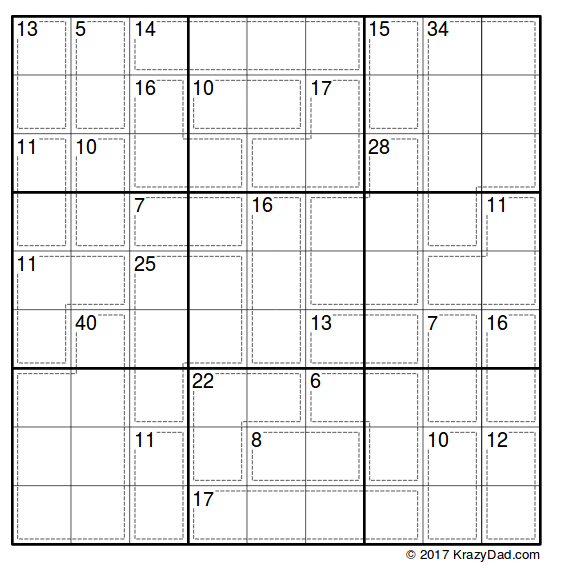
\includegraphics[scale=0.6]{puzzles/sudoku/killer/puzzle.png}
\caption{}
\end{figure}

There are ``cages'', each cage must have distinct digits,
and its sum must be equal to the number written there in a manner of crossword.
See also: \url{https://en.wikipedia.org/wiki/Killer_sudoku}.

This is also piece of cake for Z3.
% TODO \ref
I've took the same piece of code I used for usual Sudoku ( \url{...sudoku2.py} ).

\begin{lstlisting}
...

cage=[cells[0][0], cells[1][0]]
s.add(Distinct(*cage))
s.add(Sum(*cage)==13)

cage=[cells[0][1], cells[1][1]]
s.add(Distinct(*cage))
s.add(Sum(*cage)==5)

cage=[cells[0][2], cells[0][3], cells[0][4], cells[0][5]]
s.add(Distinct(*cage))
s.add(Sum(*cage)==14)

cage=[cells[0][6], cells[1][6]]
s.add(Distinct(*cage))
s.add(Sum(*cage)==15)

cage=[cells[0][7], cells[0][8], cells[1][7], cells[1][8], cells[2][7], cells[2][8], cells[3][7]]
s.add(Distinct(*cage))
s.add(Sum(*cage)==34)

cage=[cells[1][2], cells[2][2], cells[2][3]]
s.add(Distinct(*cage))
s.add(Sum(*cage)==16)

cage=[cells[1][3], cells[1][4]]
s.add(Distinct(*cage))
s.add(Sum(*cage)==10)

cage=[cells[1][5], cells[2][4], cells[2][5]]
s.add(Distinct(*cage))
s.add(Sum(*cage)==17)

cage=[cells[2][6], cells[3][5], cells[3][6], cells[4][5], cells[4][6]]
s.add(Distinct(*cage))
s.add(Sum(*cage)==28)

cage=[cells[3][2], cells[3][3]]
s.add(Distinct(*cage))
s.add(Sum(*cage)==7)

cage=[cells[3][4], cells[4][4], cells[5][4]]
s.add(Distinct(*cage))
s.add(Sum(*cage)==16)

cage=[cells[3][8], cells[4][7], cells[4][8]]
s.add(Distinct(*cage))
s.add(Sum(*cage)==11)

cage=[cells[4][0], cells[4][1], cells[5][0]]
s.add(Distinct(*cage))
s.add(Sum(*cage)==11)

cage=[cells[4][2], cells[4][3], cells[5][2], cells[5][3], cells[6][2]]
s.add(Distinct(*cage))
s.add(Sum(*cage)==25)

cage=[cells[5][1], cells[6][0], cells[6][1], cells[7][0], cells[7][1], cells[8][0], cells[8][1]]
s.add(Distinct(*cage))
s.add(Sum(*cage)==40)

cage=[cells[5][5], cells[5][6]]
s.add(Distinct(*cage))
s.add(Sum(*cage)==13)

cage=[cells[5][7], cells[6][7]]
s.add(Distinct(*cage))
s.add(Sum(*cage)==7)

cage=[cells[5][8], cells[6][8]]
s.add(Distinct(*cage))
s.add(Sum(*cage)==16)

cage=[cells[6][3], cells[6][4], cells[7][3]]
s.add(Distinct(*cage))
s.add(Sum(*cage)==22)

cage=[cells[6][5], cells[6][6], cells[7][6]]
s.add(Distinct(*cage))
s.add(Sum(*cage)==6)

cage=[cells[7][2], cells[8][2]]
s.add(Distinct(*cage))
s.add(Sum(*cage)==11)

cage=[cells[7][4], cells[7][5]]
s.add(Distinct(*cage))
s.add(Sum(*cage)==8)

cage=[cells[7][7], cells[8][7]]
s.add(Distinct(*cage))
s.add(Sum(*cage)==10)

cage=[cells[7][8], cells[8][8]]
s.add(Distinct(*cage))
s.add(Sum(*cage)==12)

cage=[cells[8][3], cells[8][4], cells[8][5], cells[8][6]]
s.add(Distinct(*cage))
s.add(Sum(*cage)==17)

...
\end{lstlisting}

( The full file: \url{...killer_sudoku.py} )

The puzzle marked as ``Super-Tough Killer Sudoku Puzzle'' (again, for humans?),
however it took $\approx 30$ seconds on my old Intel Xeon E3-1220 3.10GHz to solve it:

\begin{lstlisting}
5 3 4 7 1 2 8 9 6
8 2 1 4 6 9 7 5 3
9 6 7 8 3 5 4 2 1
2 4 6 1 9 7 3 8 5
7 1 9 3 5 8 6 4 2
3 8 5 6 2 4 9 1 7
4 7 2 5 8 3 1 6 9
6 5 8 9 7 1 2 3 4
1 9 3 2 4 6 5 7 8
\end{lstlisting}

